\openingarticle
\def\ppages{\pagerange{hughes:firstpage}{hughes:lastpage}}
\def\shorttitle{\enquote{In my sword I trust}}
\def\maintitle{\enquote{In my sword I trust}. A Reassessment of Irish Iron Age Swords With a Focus on Their Potential Use in Battle}
\def\shortauthor{Sam Hughes}
\def\authormail{sam.hughes@ucdconnect.ie}
\def\affiliation{University College Dublin}
\def\thanknote{\footnote{\href{https://ucd.academia.edu/SamHughes}{Sam Hughes} is a recent BA graduate of the School of Archaeology at University College Dublin (Ireland). His research interests lie mainly in Later European Prehistory and experimental archaeology, with a focus on Irish prehistory and ancient warfare in Europe and the Mediterranean.}}
%--------------------------------------------------------------
\mychapter{\maintitle}
\begin{center}
	{\Large\scshape\shortauthor \thanknote}\\[1em]
	\email \\%[.5em]
	\affiliation
\end{center}
\vspace{3em}
\midarticle
%--------------------------------------------------------------
\label{hughes:firstpage}
\sisetup{%
	range-phrase ={--},%
	}


%----------------------------------------------------------------------------------------
%	ABSTRACT
%----------------------------------------------------------------------------------------


	


	
\begin{myabstract}
Irish\marginnote{Abstract\\ (In French see below)} Iron Age swords are remarkable in terms of their short length compared to their contemporaries in La Tène Britain and Continental Europe, a feature that has led to speculation that they were primarily stabbing weapons or a ceremonial object not intended for fighting. This research incorporates previously published swords with new material from a survey of Irish museum databases to examine the swords in terms of blade morphology and dimension to infer their possible use in battle. The study shows that the majority of swords from the period (c.\,700 \BC – c.\,400 \AD), both La Tène and sub-Roman, have features of stabbing weapons used for fighting on foot. This is at odds with the nature of weaponry found elsewhere in La Tène Europe, and highlights an insular development in Ireland during the period. Through two case studies, this analysis also shows that in interacting with the outside world, conscious choices may have been made when it came to importing weapons and ideas. By clarifying the suggestions made in other works about the uses of these swords, this article looks at the swords from a new dimension, one that also relates these weapons to the nature of warfare and society in Iron Age Ireland.
\end{myabstract}


%----------------------------------------------------------------------------------------
%	ARTICLE CONTENTS
%----------------------------------------------------------------------------------------
\begin{quote}
\begin{flushright}
\ldots\ But because of the frequency of blows, \\
the majority of spears shattered and they\\
then engaged each other with swords.\\
{\footnotesize Diodorus Siculus, 15.86.2  }
\end{flushright}
\end{quote}
\vspace{2em}

%\section{Introduction}

\lettrine[nindent=0em,lines=3]{T}{he}  swords of the Irish Iron Age (c.\,700 BC – c.\,400 AD; fig. \ref{hughes_fig1}) are unique in terms of their remarkably short stature. They range from \SIrange[range-phrase= --]{37.5}{57.9}{\cm} in length, almost half the average of their British or Continental La Tène contemporaries (which range from \SI{60}{\cm} to over \SI{1}{\meter}). 
Research has been limited by both the low number of examples (currently less than \num{40}) and single/antiquarian nature of the finds, with only one sword from a dated context. 

\begin{wrapfigure}{O}{.5\textwidth}
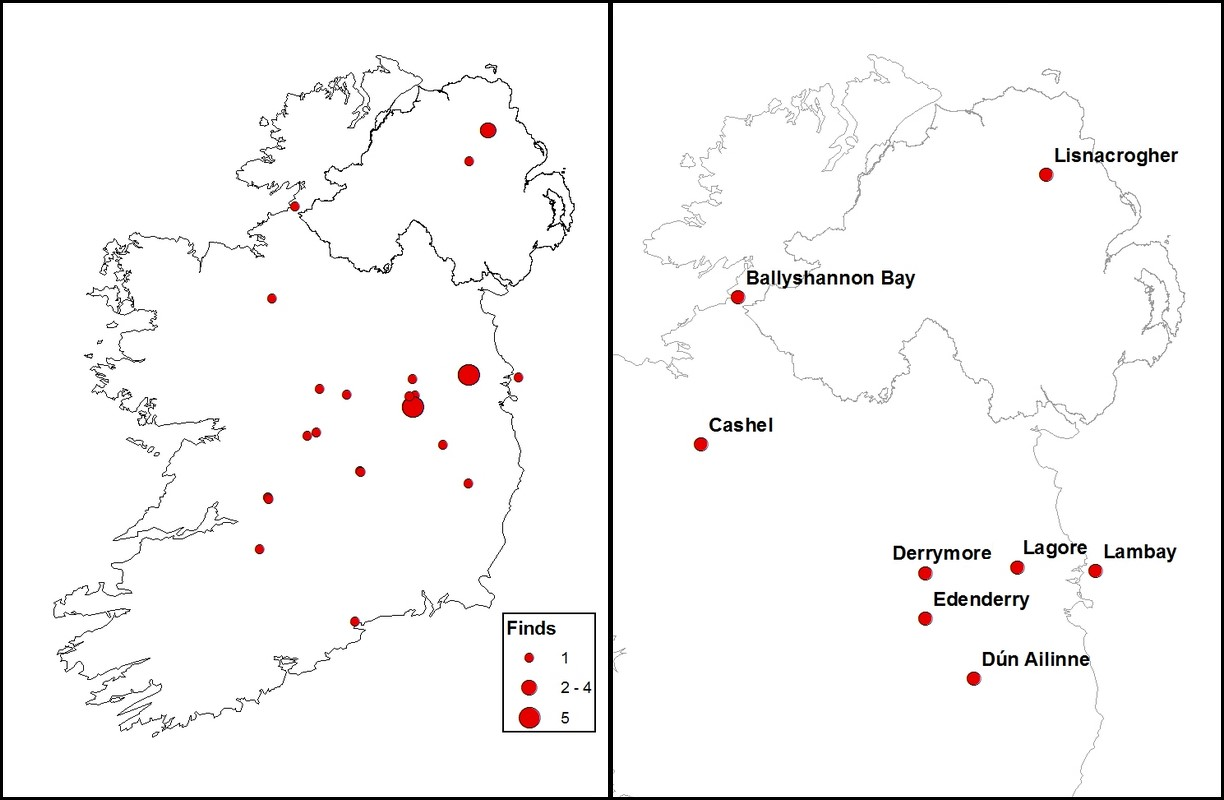
\includegraphics[width=\linewidth]{figures/Hughes_Sword_fig01.jpg} 
\caption{Distribution of Iron Age swords in Ireland and main sites mentioned in the text}
\label{hughes_fig1}
\end{wrapfigure}
Previous research on Irish Iron Age swords \parencites{Rynne1982}{Raftery1983} mainly focused on swords of La Tène type and on the creation of typologies, linking the Irish swords to the chronology of continental La Tène material. 
They excluded other types, such as the so-called ‘sub-Roman’ ones. 
Raftery’s catalogue (1983) provides a typology comprising two main groups: 
La Tène 1 and 2. La Tène 1 consists of those swords with metal hilt-guards (fig. \ref{hughes_fig2}). 
Type 2 is made up of two subgroups: 
swords with skeuomorphic representations of the metal hilt-guard (type 2A, known from only two examples), while those without falling into type 2b 
\parencite[83--106]{Raftery1983}. 
Raftery suggests that type 1 swords derive from the Middle La Tène style after De Navarro and gives the \nth{3} century BC as a possible date for their origins in Ireland 
\parencites{DeNavarro1972}[83]{Raftery1983}. 

Rynne’s \citeyear{Rynne1982} essay provides an overview of both the general European La Tène sword typology and of how Irish swords fit into this system on the basis of factors such as hilt-guard, hilt-guard mount and blade morphology as well as blade cross-section (fig. \ref{hughes_fig3}). 
Rynne’s typology defines 4 types of La Tène sword: A, B, C (all of which would be grouped into Raftery’s type 1) and Ultimate (corresponding to Raftery’s type 2). 
This progression also includes the ‘sub-roman’ type that he dates to the \nth{4}--\nth{5} centuries (1982:95).

%\begin{wrapfigure}{O}{.5\textwidth}
%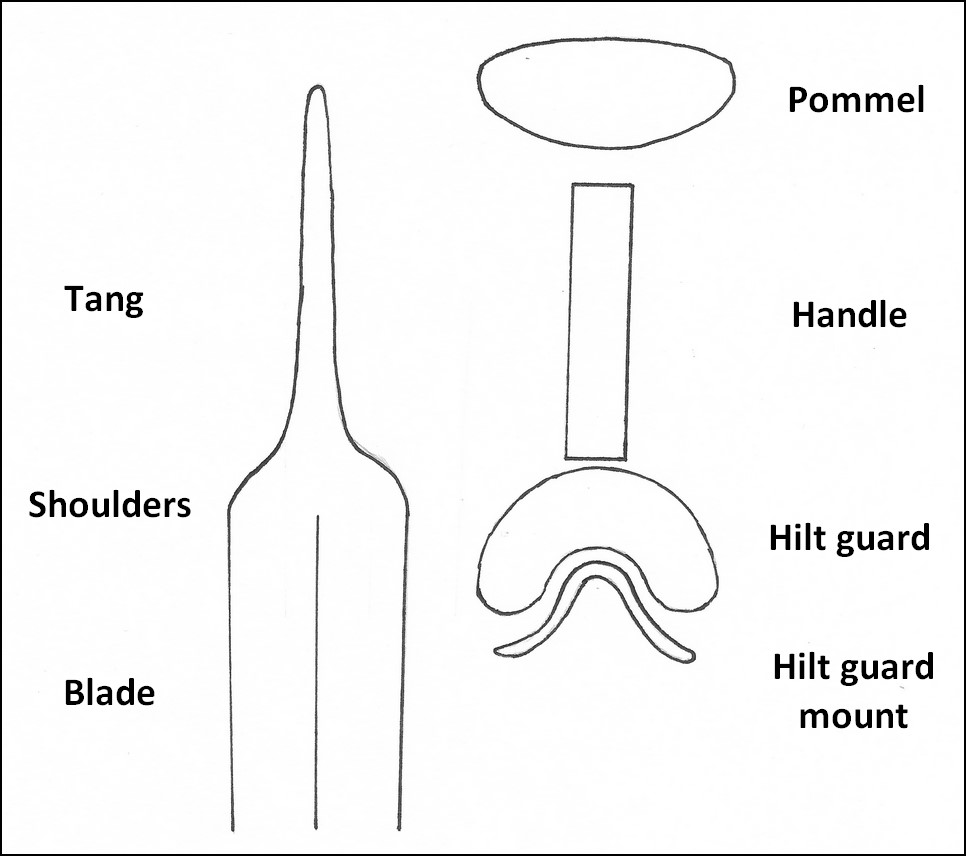
\includegraphics[width=\linewidth]{figures/Hughes_Sword_fig02.jpg} 
%\caption{Terminology of sword parts used in this paper}
%\label{hughes_fig2}
%\end{wrapfigure}

\begin{figure}[!tb]
\begin{subfigure}[b]{0.45\textwidth}
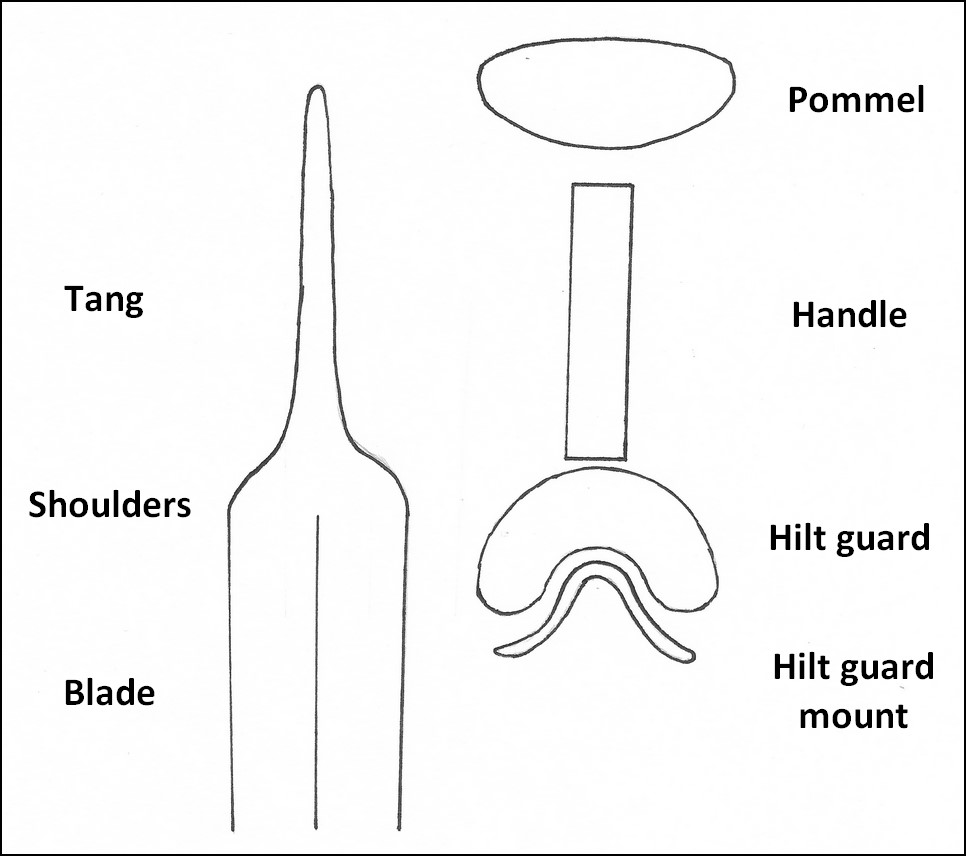
\includegraphics[width=\linewidth]{figures/Hughes_Sword_fig02.jpg} 
\caption{Terminology of sword parts used in this paper}
\label{hughes_fig2}
\end{subfigure}
\hfill
\begin{subfigure}[b]{0.45\textwidth}
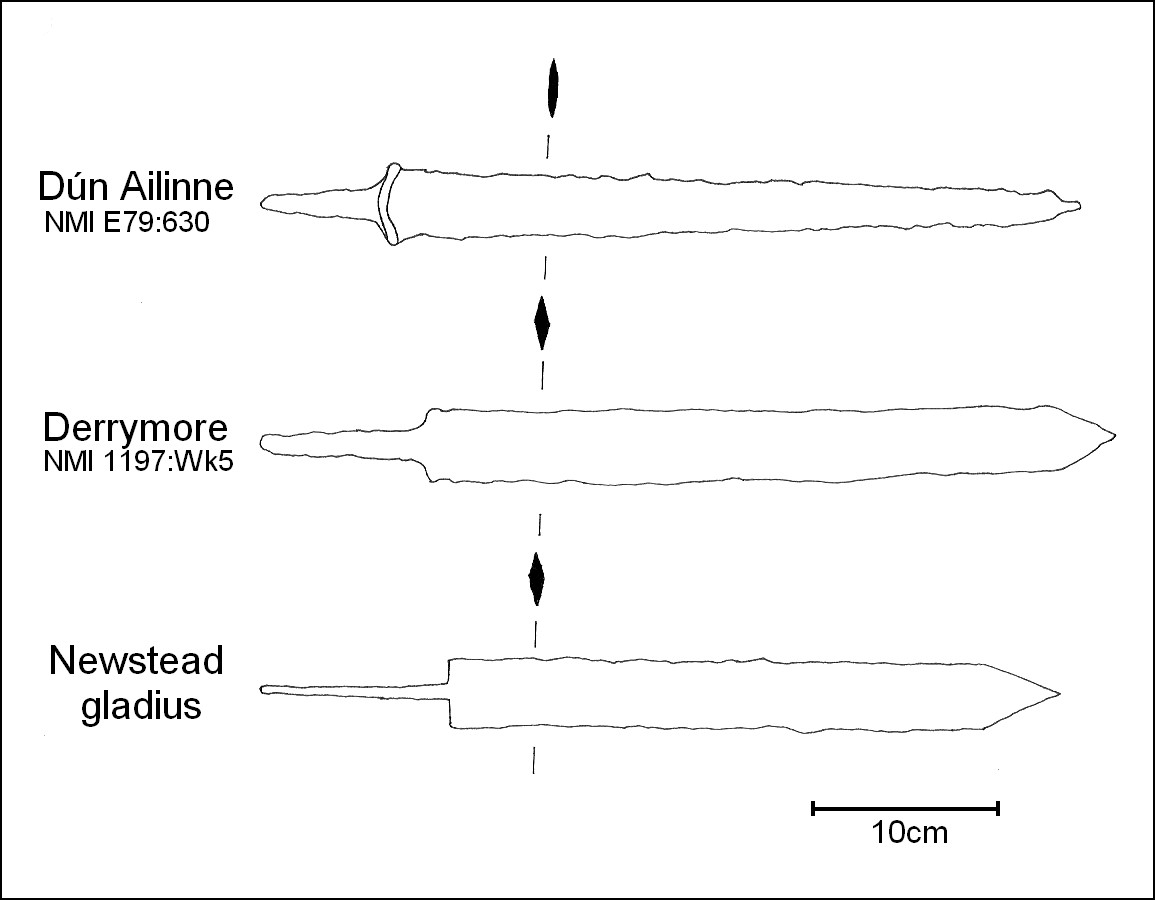
\includegraphics[width=\linewidth]{figures/Hughes_Sword_fig04.jpg} 
\caption{Three of the sword types mentioned in the texts. From top to bottom: La Tène, Sub-Roman and Pompeii Gladius types.}
\label{hughes_fig4}
\end{subfigure}
\caption{Terminology and sword types.}
\end{figure}

Both Raftery and Rynne suggest that the earliest Irish La Tène swords derive from the Middle La Tène style after De Navarro. Giving the \nth{3} century BC as a possible date for their origins in Ireland \parencites{DeNavarro1972}{Rynne1982}[83]{Raftery1983}. 
Both these classifications are, however, problematic. 
Both rely on hilt-guard morphology to provide a relative chronology -- which is in keeping with approaches to La Tène swords elsewhere in Europe 
\parencites(e.g.)(){DeNavarro1972}{Stead2006} -- but many swords in Ireland are found without hilt fittings. 
Rynne’s blade-type progression has also been thrown into question by the dating of the Dún Ailinne sword (see fig. \ref{hughes_fig4}): 
it would be classified as type A (\nth{3}/\nth{2} centuries BC) but it comes from a context dated to the \nth{1} century AD \parencite[88\psq]{Johnston2007}. 
As Raftery’s La Tène typology is broader and lacks the chronological issues of Rynne’s, I have chosen to use it to classify the swords which I examined in the museum and that are not included in his catalogue \parencite{Raftery1983} (see appendix 1).

\begin{wrapfigure}{O}{.5\textwidth}
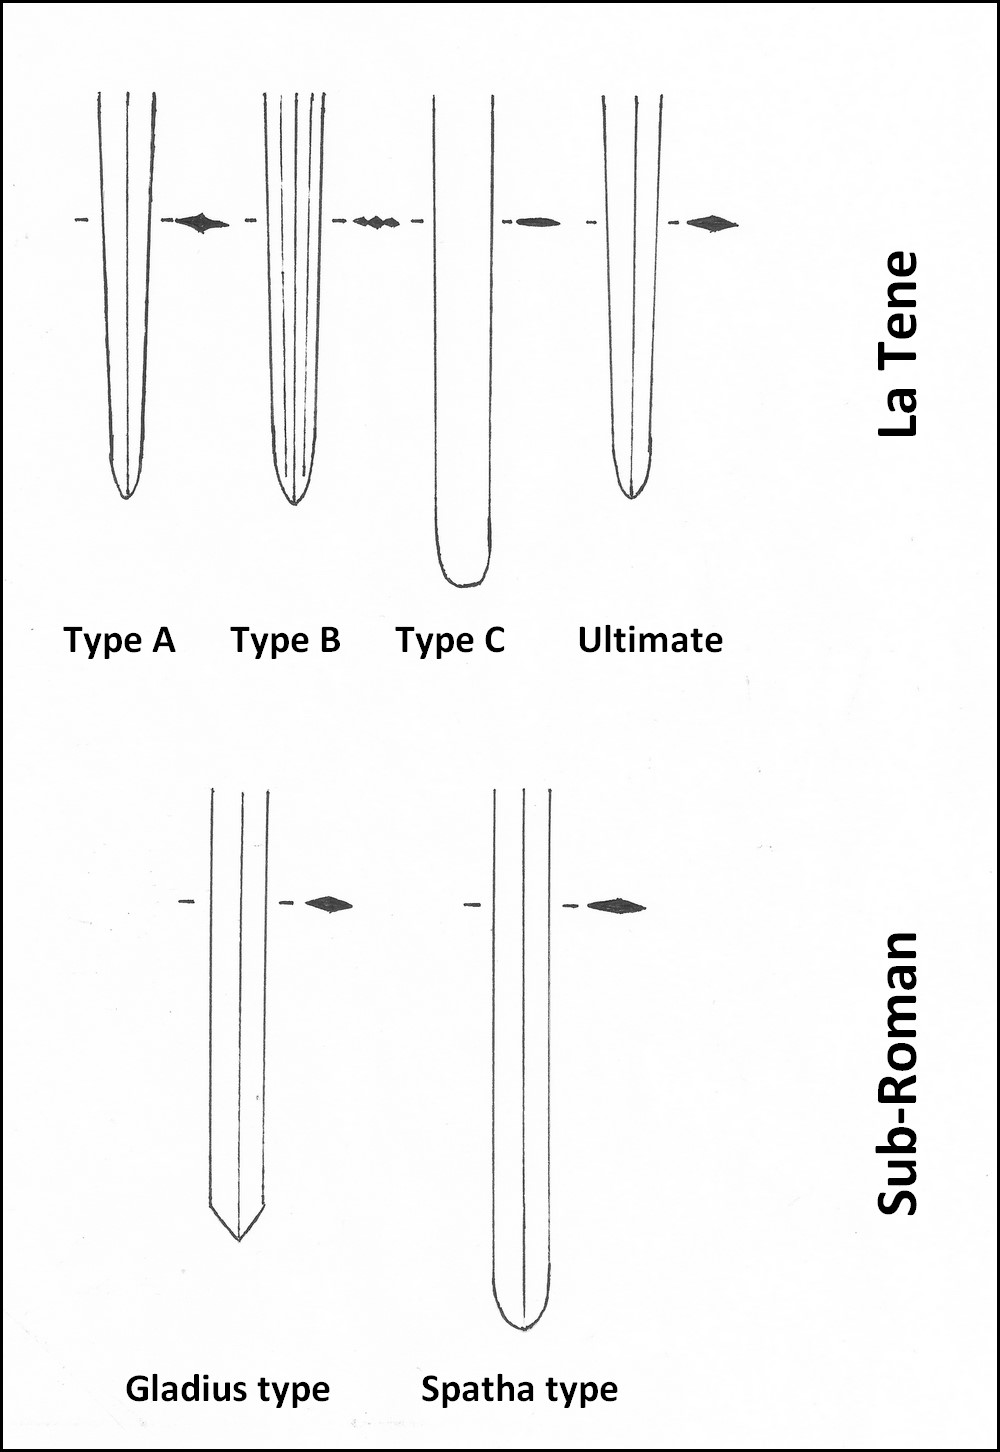
\includegraphics[width=\linewidth]{figures/Hughes_Sword_fig03.jpg} 
\caption{Rynne's typology of Iron Age swords \parencite[after][]{Rynne1976}}
\label{hughes_fig3}
\end{wrapfigure}

Other than the typological work described above, metallurgical analysis on six Irish Iron Age swords was carried out by \textcite{Scott1990} as part of a wider analysis of early ironworking in Ireland. 
This analysis reveals that there was an entire spectrum of metalworking quality when it came to sword manufacture. 
Some would have been an “ineffective weapon” \parencite[125]{Scott1990}, while others, such as an example from Lisnacrogher, Co Antrim, were finely made with a skill that matched that of the decorated bronze scabbards found with them \parencite[65]{Scott1990}.
The research presented here considers various aspects of these weapons in order to question how the Irish Iron Age sword may have functioned in battle. 
Previous works have speculated as to the possible applications of this weapon. 
\textcite[121]{Raftery1989} suggests that stabbing is the main use these weapons would have had. 

It has also been put forward that such weapons may not have been intended for use in battle, and that warfare may have been “... a ritual farce” \parencite[304]{Waddell2000}. 
\textcite{Pleiner1993} brings together morphological, metallurgical as well as written evidence for Iron Age swords in Europe to discuss an overarching ‘Celtic’ sword and fighting style: 
one of long slashing swords. He assumes this fighting style must have survived longer in Ireland; 
the island having never been subdued by Rome \parencite[165]{Pleiner1993} but this suggestion does not take into account the uniquely short length of Irish swords.
Since the last comprehensive catalogue of these artefacts was carried out in 1983 as part of Raftery’s Catalogue, 
later works such as \citetitle{Pleiner1993}  and Mallory’s \citetitle{Mallory2013} were consulted to focus on compiling a list of any discovered after the creation of Raftery’s Catalogue. 
Apart from Scott’s 1990 metallurgical study that revealed two swords, information about the number of IA swords in Ireland was usually a statement that they numbered c. \num{30} 
\parencite[e.g.][180]{Mallory2013}. 

%\begin{wrapfigure}{O}{.5\textwidth}
%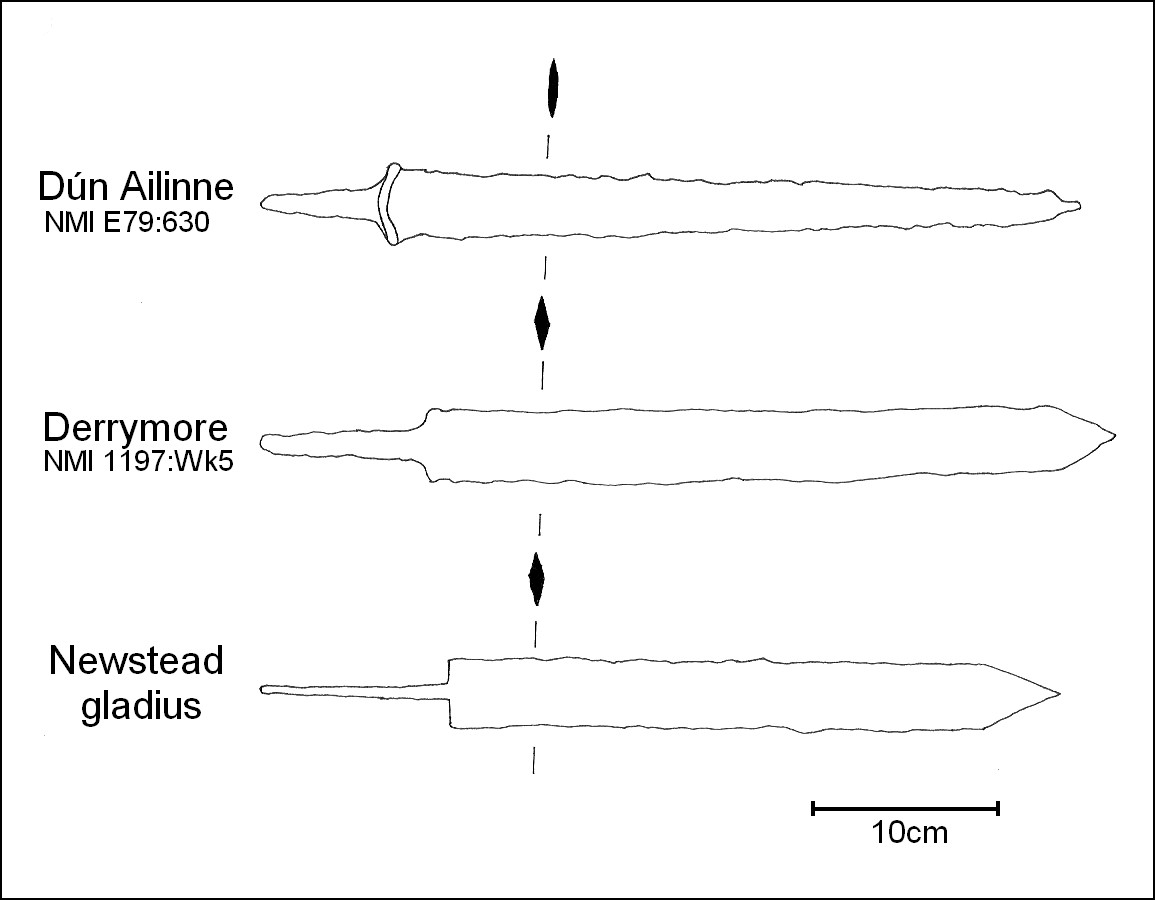
\includegraphics[width=\linewidth]{figures/Hughes_Sword_fig04.jpg} 
%\caption{Three of the sword types mentioned in the texts. From top to bottom: La Tène, Sub-Roman and Pompeii Gladius types.}
%\label{hughes_fig4}
%\end{wrapfigure}
In order to bridge this gap in numbers I contacted the National Museum of Ireland and the Ulster Museum in Belfast. 
Through a survey of the National Museum’s topographical files the number of swords under study was brought up to 38. 
All relevant swords in the Ulster Museum were recorded in the Catalogue; 
however, a fragment of a sword that had been lodged in its scabbard had since been removed. 
Work on the swords from this period has also concentrated almost entirely on swords of La Tène type, however, this study also includes five swords of so-called “sub-Roman” type. 
The reasons for this inclusion will be discussed in more detail below.


As\marginnote{The Swords} mentioned above, this project differs from previous studies in that it includes the so-called “sub-Roman” swords, traditionally excluded from the corpus of Irish material. However, recent research has led to the acceptance of Romano-British and other non-La Tène material as being an integral part of the Irish Iron age 
\parentext{for a more in-depth discussion on the treatment of “intrusive” material during the Irish Iron Age \cite[see][22\psqq]{CahillWilson2014}}. 
\textcite[95]{Rynne1982} considers these ‘sub-Roman’ swords to have appeared in Ireland in the \nth{4}/\nth{5} centuries AD, 
when Irish colonies were set up in Wales.

This was based on the general assumption that there was no interaction with the Roman Empire during the first four centuries AD. 
However the work of the Late Iron Age and Early ‘Roman’ Ireland Project has shown that there was indeed contact during this period 
\parencite[esp. chapters 7--8]{CahillWilson2014}, 
and this provides the basis for the inclusion of ‘sub-Roman’ material into the present analysis. 
The assemblage under study consists of 38 swords in varying states of preservation. 
Of these 38 swords, 25 are of La Tène type, 5 of sub-Roman type and 8 could not be classified (see appendix 1). 
I shall now briefly present some of the most significant – and well-documented - swords under study. 
The sword from Dún Ailinne, Co Kildare, is unique in that is the only known Irish La Tène sword from a dated context. 
Until the time of this study it was also the only sword known to have an iron rather than copper alloy hilt-guard mount 
\parencite[88\psq]{Johnston2007}. 

During my visit to the National Museum however, I identified a similar hilt-guard on the sword NMI 1989:86 (appendix 1). 
The sword was found against the side of a palisade trench and it is suggested that it was a foundational deposit for the ‘Mauve’ phase structure, 
dated to the \nth{1} century AD \parencite[89]{Johnston2007}.
There is also the possibility this was a votive deposit in the trench, although this would be an unusual circumstance for such an offering \parencite[89]{Johnston2007}.
The anthropoid sword hilt from Ballyshannon bay in Co. Donegal (fig. \ref{hughes_fig5}) belongs to a small subgroup of La Tène swords found all across Europe. 
This type is named after the configuration of the one-piece bronze or iron hilt into a stylized human body. 
There are anywhere up to 90 examples of these swords in Europe ranging from Early to Late La Tène periods \parencite[193]{OBrien2009}. 
Their blades measure between \SI{29}{\cm} and \SI{55}{\cm}. 
Unlike the parallel-sided longer La Tène swords mentioned above, these swords generally taper to a point across their entire length. 
Within the typology of these swords the Ballyshannon hilt is categorized as type G, dating to c.\,150 BC – AD 50 \parencite[193]{OBrien2009}. 
It is also noted that the closest parallels for the Irish example are from southern France and it is almost certainly imported 
\parencites[193]{OBrien2009}[143]{Raftery1994}[25]{CahillWilson2014}. 
In general, because of its shorter blade, this type is often interpreted as having a primarily ceremonial or ritual function, 
with its potential as a weapon being doubted \parencites[69]{Pleiner1993}[160]{Lejars2007}.

\begin{wrapfigure}{O}{.5\textwidth}
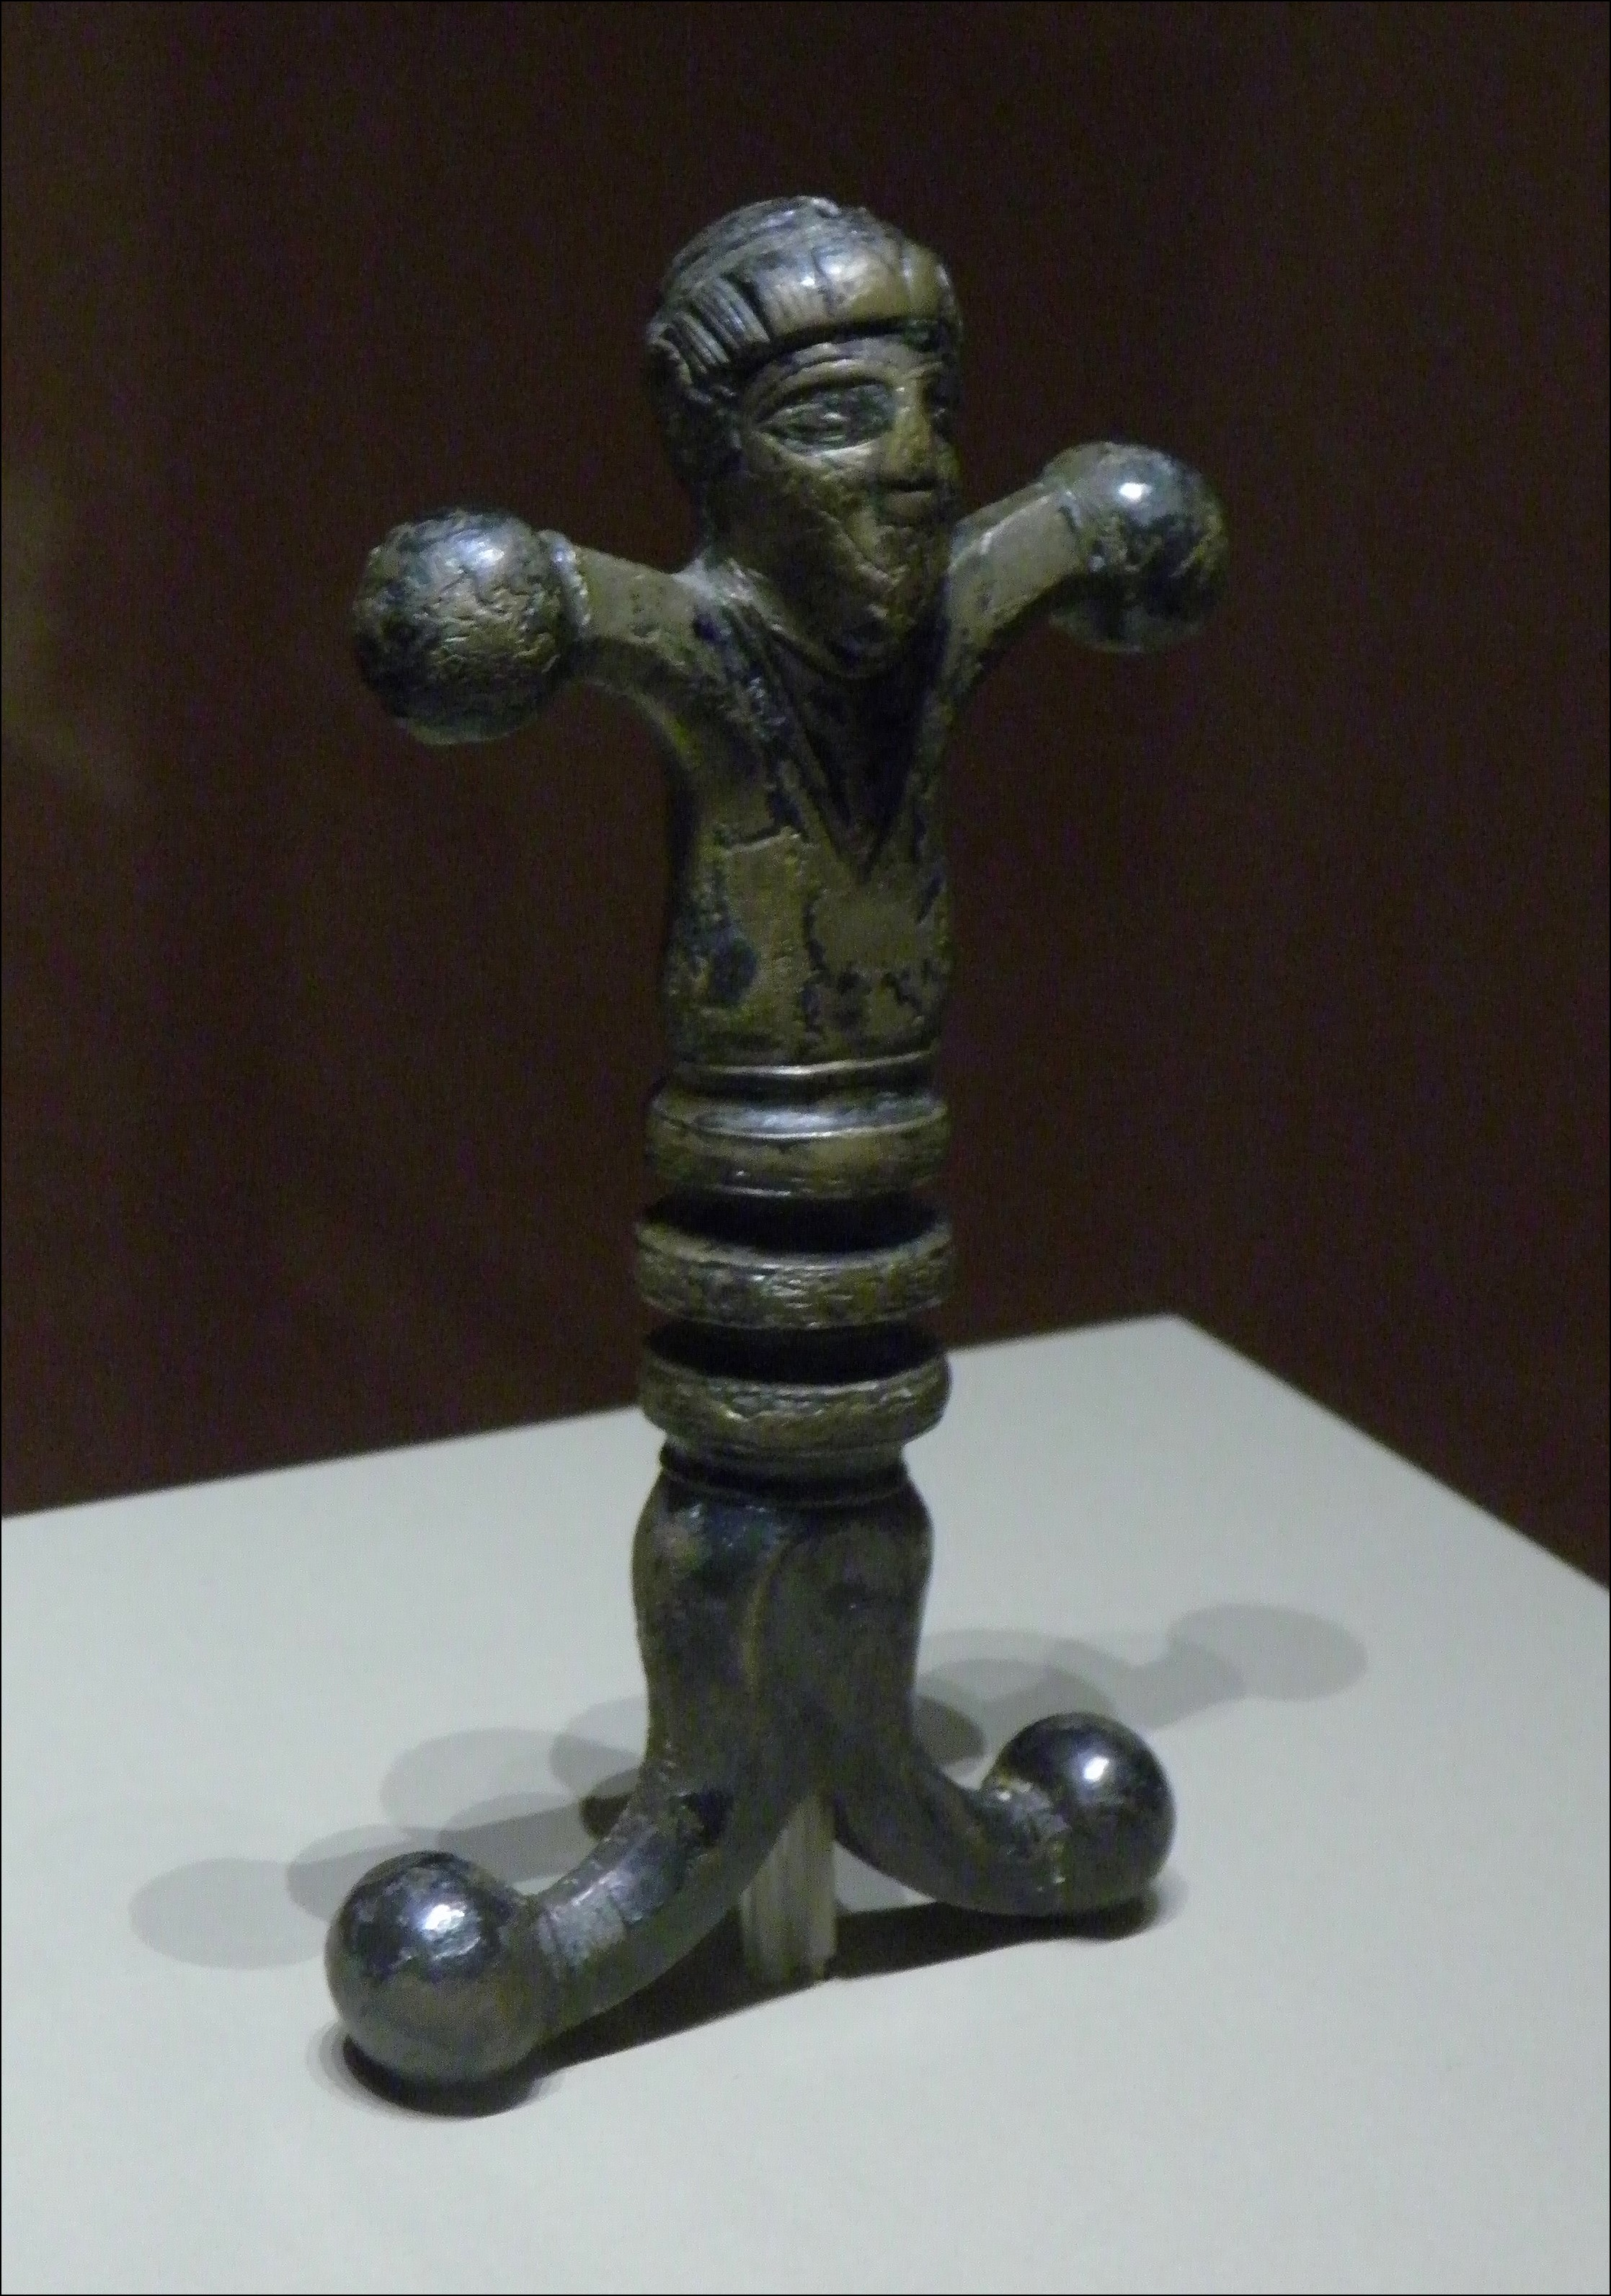
\includegraphics[width=\linewidth]{figures/Hughes_Sword_fig05.jpg} 
\caption{Anthropomorphic handle from Ballyshannon Bay © Hughes 2015}
\label{hughes_fig5}
\end{wrapfigure}
The final group of swords that need to be reviewed here are the examples of sub-Roman type from Lagore Crannóg, Co Meath. 
The crannóg itself is said to have been occupied between the \nth{7} and \nth{10} centuries, 
a date that the excavator based on chronological information provided by
 early medieval records known as the Annals rather than on scientific methods \parencite[6]{Hencken1950}. 
 This dating has since then been questioned and his chronology of the site, especially of the early layers, 
 has been challenged on several occasions \parencites(e.g.)(){Lynn1985-6}[77\psqq]{CahillWilson2010}.  
 The human remains recovered from the site of the crannóg have now been dated and a group of them belong to the Bronze and to the Iron Age, 
 providing evidence for a significant prehistoric horizon at Lagore 
 \parencite[32\psqq]{Carty2013}; see also \textcite{Gugliemi}, for a reassessment of the Roman and Iron Age material at Lagore). 
 Two swords are noted by Hencken to have affinities with the Roman \emph{gladius} and \emph{spatha} types \parencite[91; sword numbers 0002:Wk002 and 0003:Wk003, appendix 1]{Hencken1950}
  and research by the Discovery Programme’s Late Iron Age and ‘Roman’ Ireland project has found a parallel between the longer ‘\emph{spatha}’ from Lagore (0002:Wk002) and Roman swords from the Danish site of Illerup Ådal \parencite[28]{CahillWilson2014}. 
  Unfortunately, the Lagore examples are antiquarian finds and the context of their deposition is unknown.
The rest of the swords under study are single finds with limited or no information regarding their contexts from which they were recovered. 
The most extreme case is the one from Cashel, Co. Sligo which was found in “the thatch of a derelict cottage” \parencite[92]{Raftery1983}.

%\subsection{The sword as a weapon}
For\marginnote{The sword as a weapon} the present research, it is the blade morphology and especially the cross section that are the main focus of analysis. 
By examining their dimensions, their relation to contemporary swords from Britain and the Continent and discussing their place in relation to the rest of the Irish Iron Age ‘warrior panoply’, some light can be shed on the way in which Irish Iron Age swords may have been used as weapons. 
Blade morphologies have an effect on the way the blade behaves in combat and can allow us to make inferences about the fighting techniques the weapon was constructed to suit. 
Of the 38 swords in the assemblage under study, only 31 were preserved well enough so that the cross-section could be identified. 
Irish Iron Age swords can be divided into four groups based on their cross section morphology (table \ref{tab1}): lozenge, midrib, lenticular and grooved/expanded-edge midrib (fig. \ref{hughes_fig6}). 




\begin{wrapfigure}{O}{.5\textwidth}
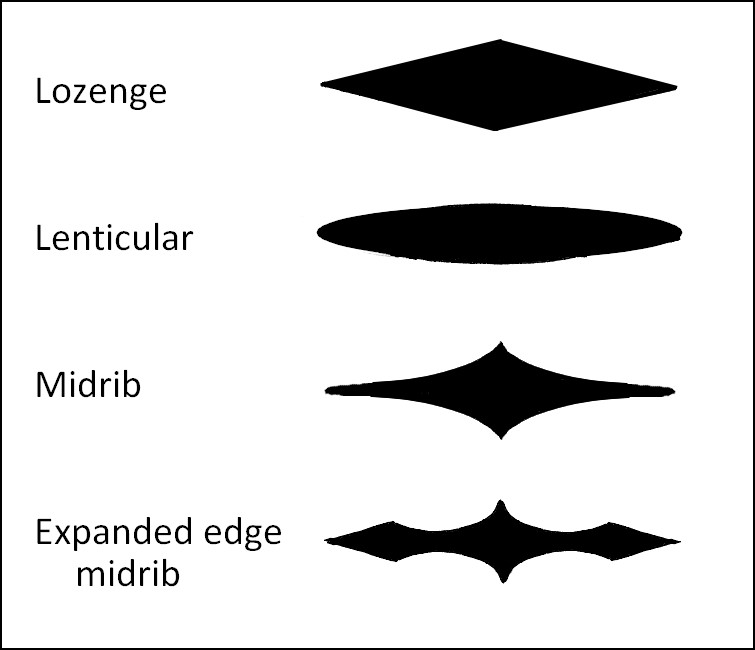
\includegraphics[width=\linewidth]{figures/Hughes_Sword_fig06.jpg} 
\caption{Blade cross-sections found in Irish Iron Age swords }
\label{hughes_fig6}
\end{wrapfigure}

\begin{figure}%{O}{.5\textwidth}
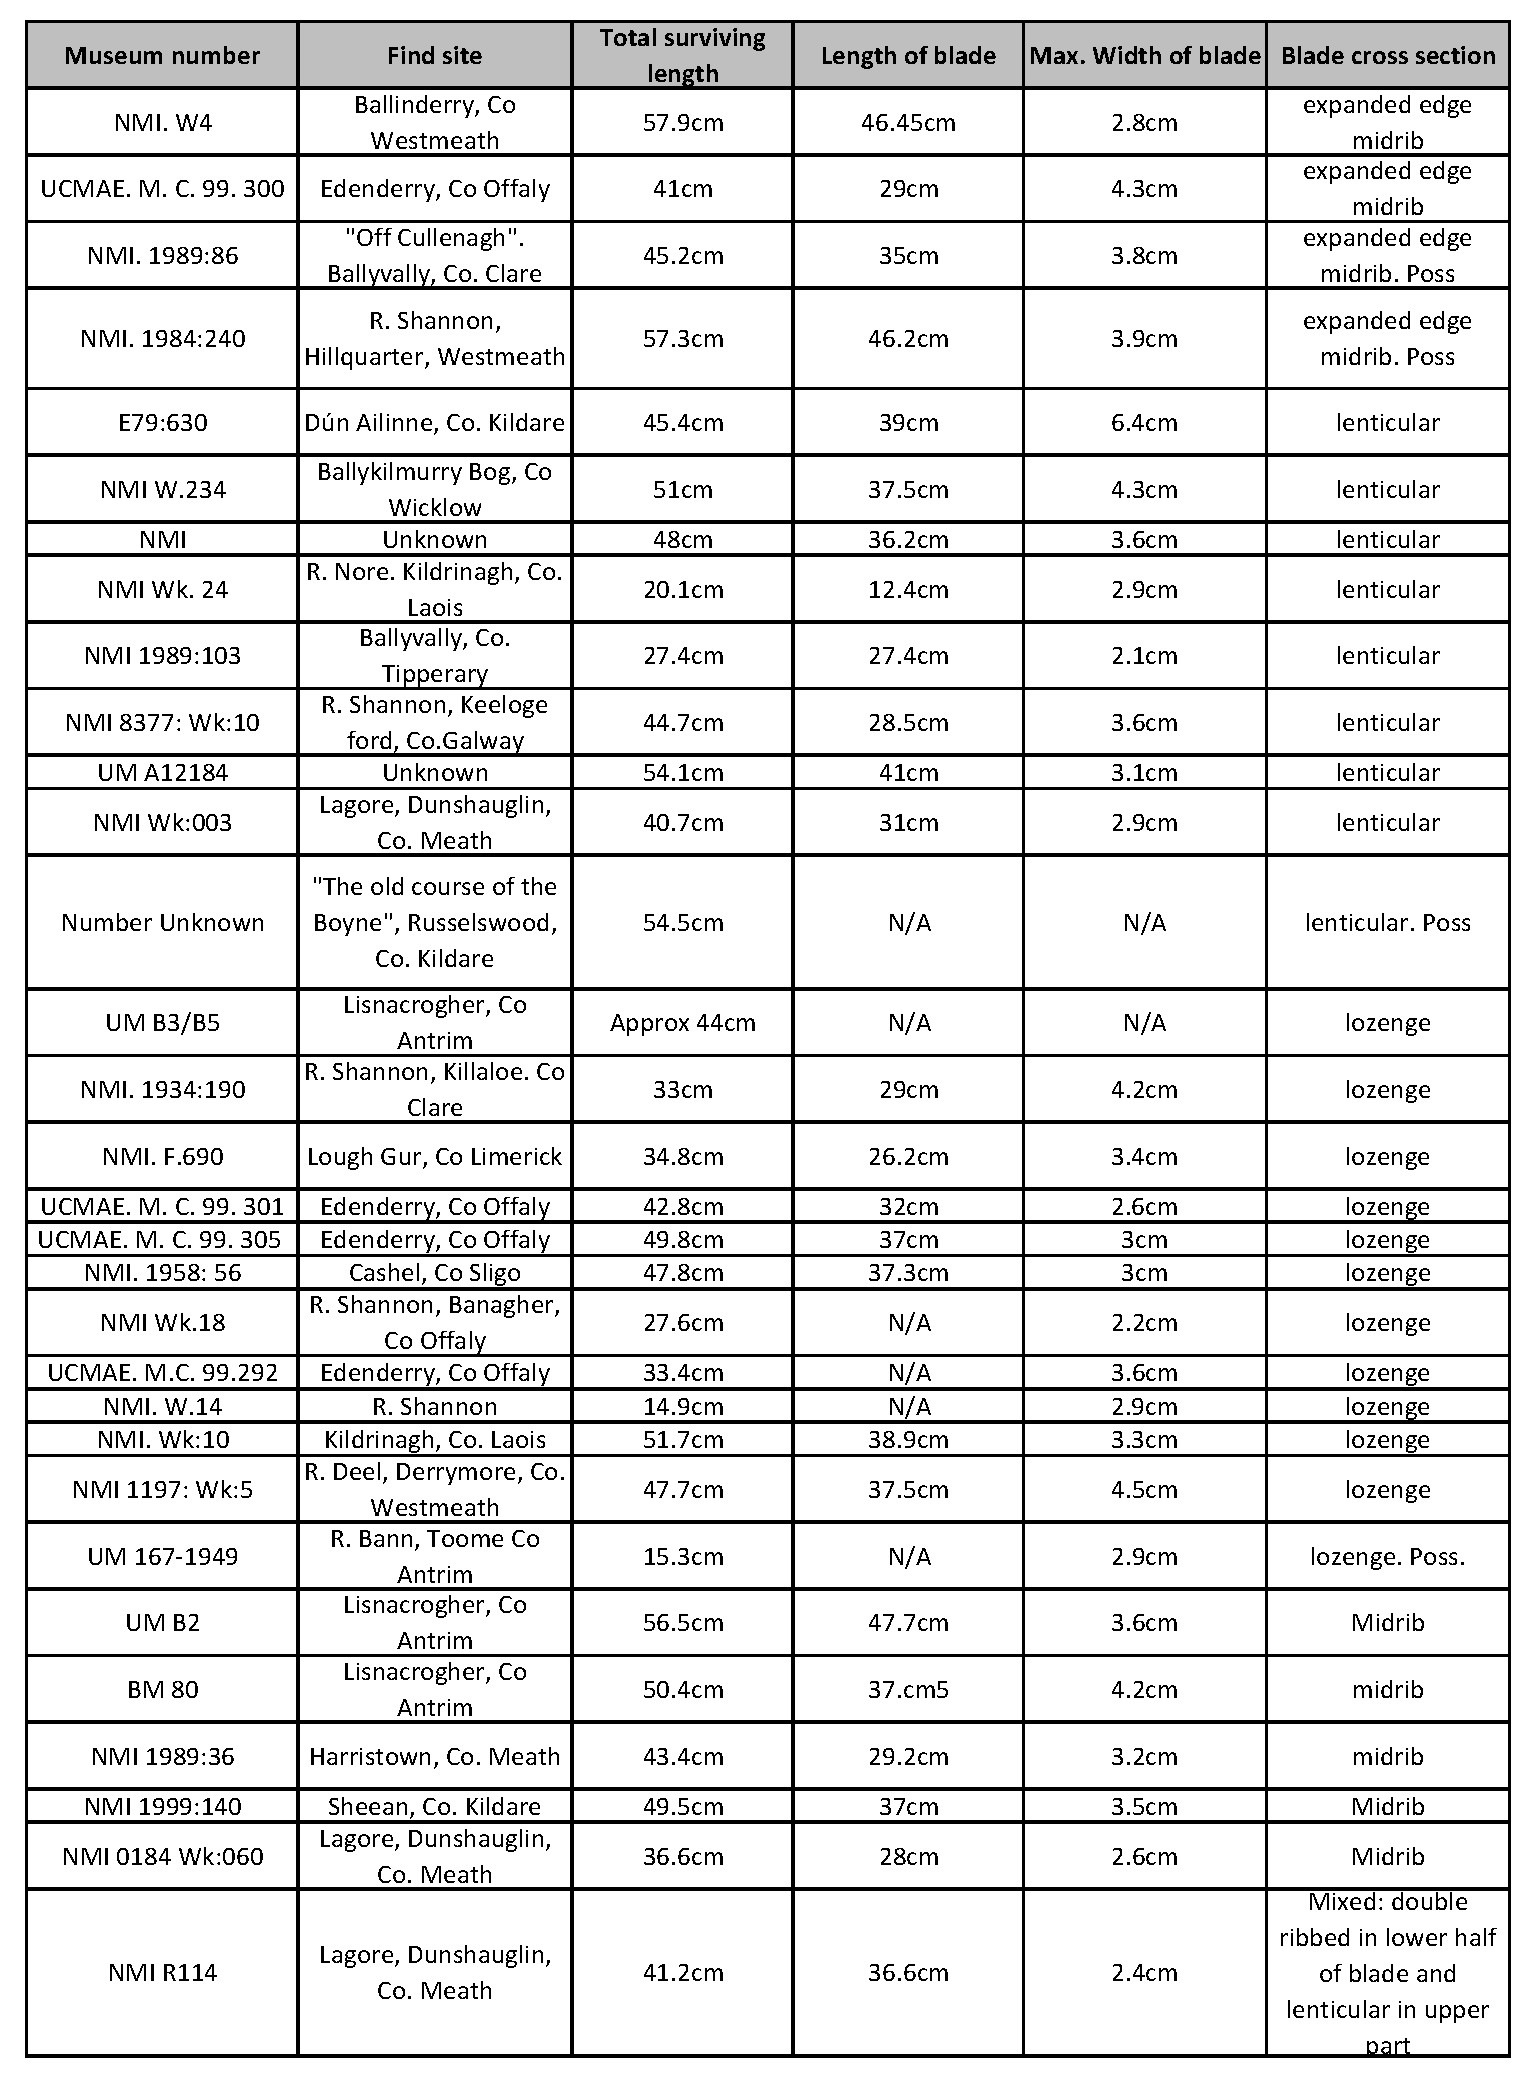
\includegraphics[width=\linewidth]{figures/Hughes_Sword_tab01.jpg} 
\captionof{table}{Cross sections of swords under study (when preserved)}
\label{tab1}
\end{figure}

	

The largest group of swords by cross-section type are those swords with a lozenge (or diamond) shaped cross-section. 
Lozenge shaped cross-sections have the effect of stiffening and strengthening the blade, a quality that increases in importance the longer the blade \parencite[106]{Inall2009}:
Inall considers lozenge shaped cross-sections as imparting less strength than midribs. 
However, it is noted by \textcite{Oakeshott1960} that in the \nth{13} century AD, European longswords developed thick lozenge shaped profiles. 
This was in response to the evolution of better plate armour at the time, which required a thrusting rather than cutting blow to defeat \parencite[301]{Oakeshott1960}. 
We can imagine that the thicker the diamond, the more rigidity it would impart to the blade, although only experimental study would reveal its relative merits. 
In total, eleven of the thirty-one swords where cross-sections can be determined are of the lozenge-shaped type.
The next largest group of swords are those with a lenticular cross-section. 
This type of blade provides the least amount of rigidity and while it could be considered an indication of poor construction, 
it does impart an advantage when using the blade as a cutting weapon \parencite[106]{Inall2009}. 
In experiments with Aegean Bronze Age swords, it was noted by \textcite[124]{Molloy2008} that the presence of a central ridge was an encumbrance when cutting. 
The advantage that this lack of upstanding features provides when cutting makes the sword a less effective thrusting weapon, a fact noted by \textcite[54\psqq]{Oakeshott1960} in relation to later continental La Tène swords. 
Seven out of thirty-one swords with identifiable cross-sections were lenticular. It is also interesting to note that where the sword was mostly intact, it can be seen that La Tène swords with this type of cross section are among the longest of the type.
Swords with a midrib number four out of the thirty-one swords under study. 

As mentioned above, Inall considers this to be the strongest type of blade section in terms of ability to resist impact on end of a blade, 
such as when using a weapon for thrusting attacks \parencite[106]{Inall2009}. 
This is at the expense of the blade becoming less effective at cutting.
The smallest group of swords with an identifiable cross-section type are those with expanded edges and a midrib. 
In British La Tène swords this is considered a later development \parencite[9]{Stead2006} and is rare in La Tène swords overall \parencite[61]{Pleiner1993}. 
This design offers the strength of the midrib while also allowing the removal of some material, creating a lighter blade.
The length of the blade is also an important factor when considering how a weapon was used. 
A short sword necessarily requires one to be close to their opponent, while a longer sword requires more distance. 
Additionally, when using a cutting or slashing attack the optimal point of impact is the final third of the blade, 
meaning enough distance to allow this must be maintained \parencite[104\psq]{Inall2009}. 

The short stature of Irish Iron Age swords has led to the suggestion that they were a stabbing and thrusting, rather than cutting or slashing, weapon \parencites[121]{Raftery1989}[142]{Raftery1994}.
Although it should be noted that it is rare for a weapon to be designed purely for one type of attacking motion \parencite[168\psqq]{Clements2007}. 
Furthermore, unlike their continental counterparts, which do vary in length over time \parencites(for a detailed study c.f.)()[50\psqq]{Brunaux2004}[159--161]{Lejars2007}, 
the Irish swords do not show such a pattern (see fig. \ref{hughes_fig7}). 

%\begin{wrapfigure}{O}{.5\textwidth}
%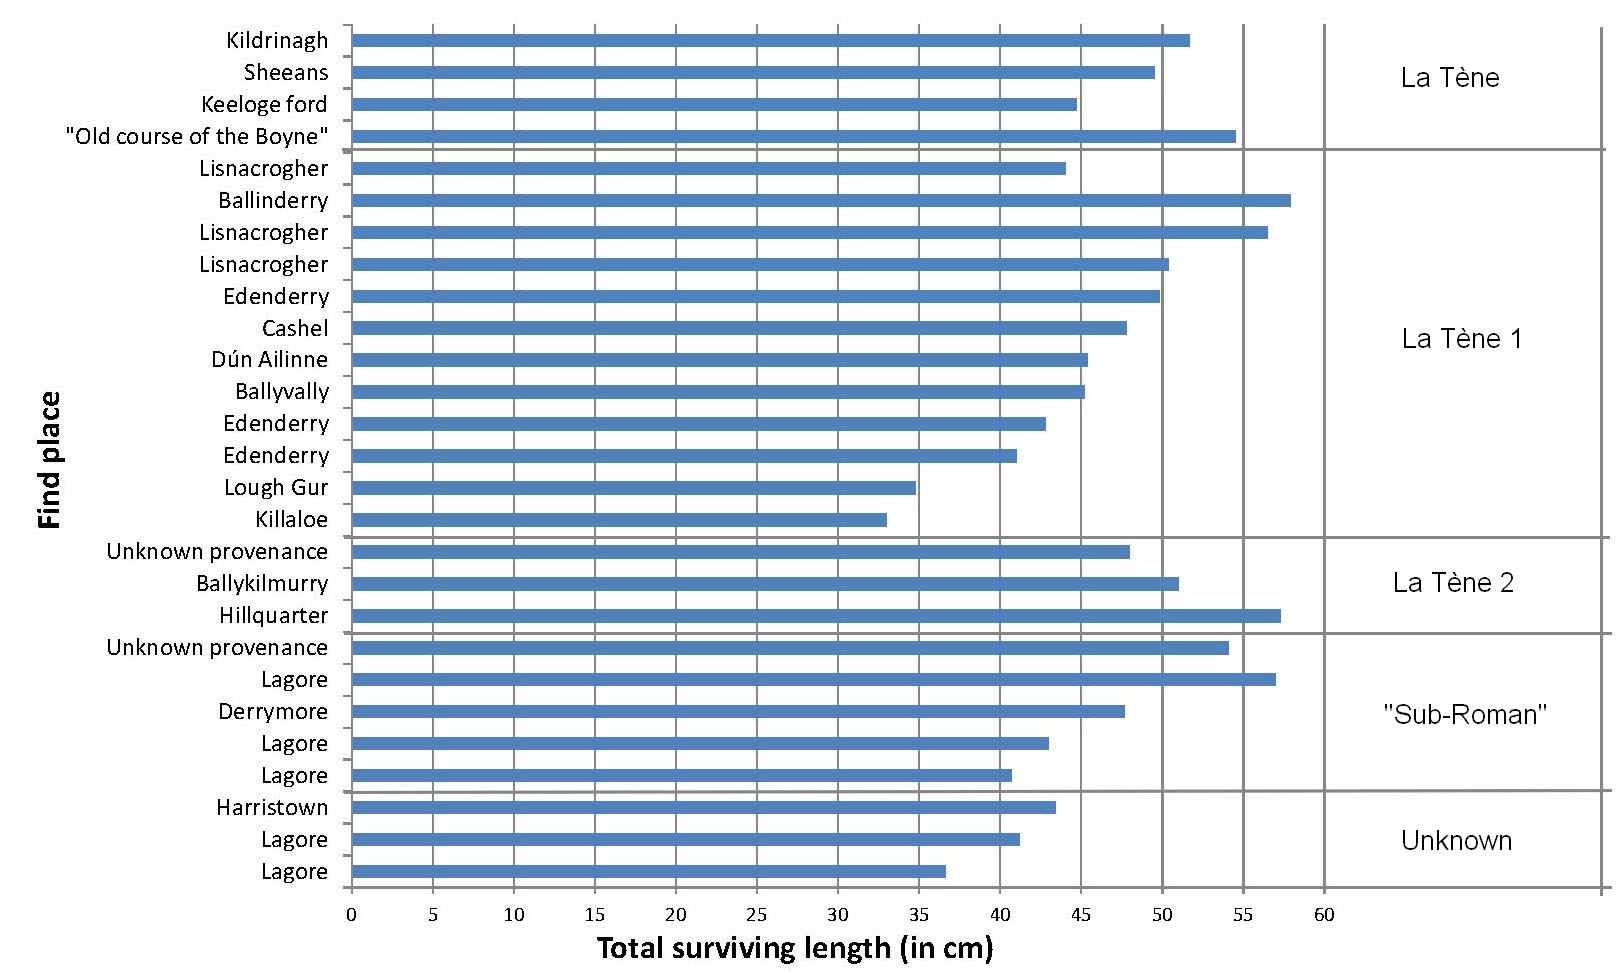
\includegraphics[width=\linewidth]{figures/Hughes_Sword_fig07.jpg} 
%\caption{Length of complete swords in study}
%\label{hughes_fig7}
%\end{wrapfigure}

\begin{figure}[!tb]%{O}{.5\textwidth}
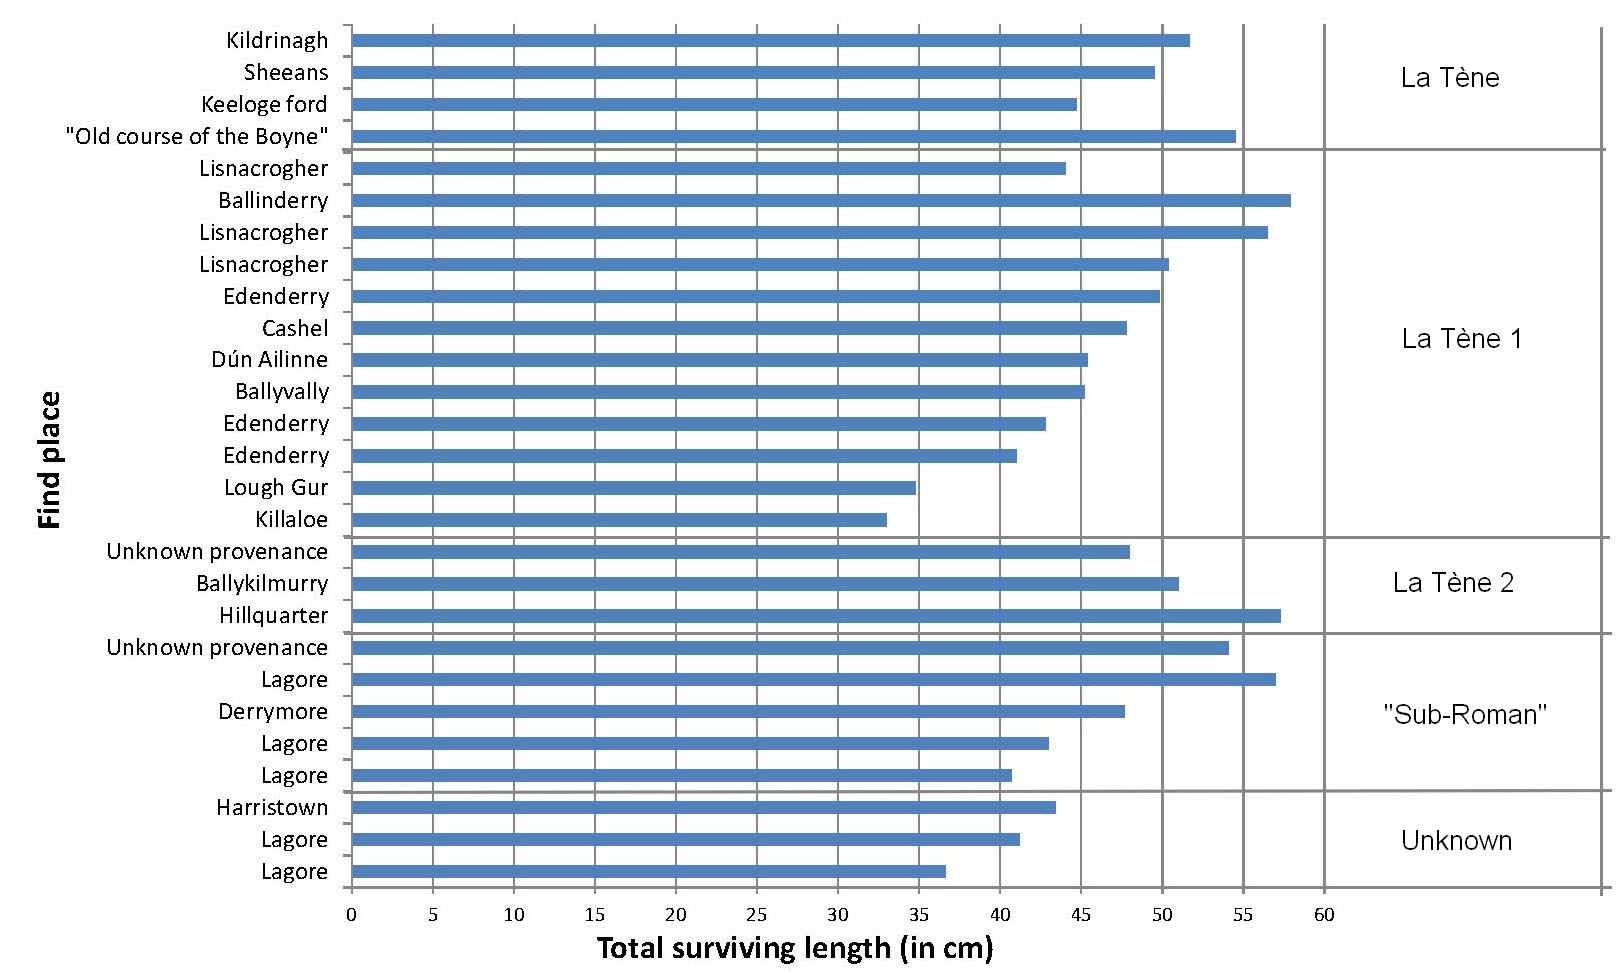
\includegraphics[width=\linewidth]{figures/Hughes_Sword_fig07.jpg} 
\caption{Length of complete swords in study}
\label{hughes_fig7}
\end{figure}

I believe that we can strengthen the argument that the Irish weapons were indeed intended as a thrust-and-cut weapon, 
rather than a cut-and-thrust weapon as many of the longer continental La Tène swords appear to be. 
Apart from length and the large proportion of Irish swords with a cross-section that lends itself to resisting pressure when thrusting, 
other features that indicate a weapon designed for thrusting are present in these swords. 
The first is the point. 
Almost all the swords under study, where the point of the blade was not broken, culminate in a fine point. 
The only exceptions are the sword described by \textcite[92]{Hencken1950} as originating from “...the old course of the Boyne”  and possibly the sword UCMAE 99.300, from Edenderry, Co. Offaly: both have rounded points. 
However, it is interesting to note that in the case of the sword from the old course of the Boyne it is among the longest examples of a La Tène sword from Ireland at \SI{54.7}{\cm} \parencites[92]{Hencken1950}[93]{Rynne1982}[91]{Raftery1983}. 
Two of the Sub- Roman Swords from Lagore also appear to have had rounded points and they will be discussed below.
When we compare these swords to their contemporaries, we see that on the continent, there was a continuous shift towards long swords that does not appear to have been present in the Irish material. 

Continental swords from La Tène I can range from \SIrange{50}{70}{\cm} and by La Tène III measuring \SIrange{80}{90}{\cm} with examples reaching lengths of \SI{1.01}{\meter} in length \parencites{Pleiner1993}[84, 264, 272, 293, 296]{Stead2006a}[159--161]{Lejars2007}. 
\textcite[50\psq]{Brunaux2004} describes the morphology of early continental La Tène swords as infantry weapons perhaps used for dueling. 
However, Middle La Tène continental sword design favours the blade over the point and being used from a position of height, such as a chariot or from horseback. 
This type of usage is also supported by the appearance in the archaeological record of sword-chains, which held the weapon in an advantageous position for riding when not in use.
This situation is mirrored in Britain, where the short type i swords evolve from \SI{65.5}{\cm} maximum to type v examples that can exceed \SI{85}{\cm} \parencite[8\psq]{Stead2006}. 
The longest swords from La Tène III can feature the expanded-edge with central midrib in order to add strength, however most are lenticular in section and there are examples of weapons over a metre in length with a lenticular cross-section. Later long swords also develop a more rounded point. 
All these features are indicative of a weapon intended for slashing and cutting \parencites[8]{Stead2006}[160]{Lejars2007}. 
Though this evolution toward long slashing swords is present in both continental and British swords, \textcite[160]{Lejars2007} stresses that shorter swords (c. \SI{65}{\cm}) were in use concurrently with the longer type, particularly from the \nth{3} century\BC onwards. 

In his view this probably represents the differing equipment of cavalry and infantry.
The Sub-Roman category of swords relate to their continental counterparts in a different way to the La Tène types. 
The swords in this study are by no means a representative sample of this type but some information about their use and origins will be discussed here. 
The two Roman military swords influence these types: the \emph{gladius}, the short, thrusting sword of the Republican and early imperial infantry, and the \emph{spatha}, the long slashing weapon of the cavalry. 
The \emph{spatha} eventually superseded the \emph{gladius} in the infantryman’s arsenal as the Roman military changed format between the late\nth{2} and early \nth{3} century AD \parencites[61]{Stephenson1999}[212\psq]{Southern2007}.
The ‘Pompeii’ type \emph{gladius} is the sword that closely matches two of the swords under study. 
In comparison to La Tène swords, this type is defined by ‘squared off’ shoulders where the blade meets the tang, they have a strong lozenge-shaped section and the blade edges are parallel before narrowing to a triangular point (see fig. \ref{hughes_fig4}). 
Unlike Irish La Tène swords, ‘Irish gladii’ are well within the typical size range for their continental relatives, which is between \SI{36.7}{\cm} and \SI{59}{\cm} \parencites[200]{Lang1988}[37]{Coulston2007}. 

The sub-Roman sword from Derrymore is \SI{47.7}{\cm} long, for example, 
and the \emph{gladius} from the fort of Newstead in Britain is \SI{43.1}{\cm} long (see fig. \ref{hughes_fig4} for a comparison between these two swords). 
There are also ‘Irish editions’ of the \emph{spatha}: An example from Lagore (0002 Wk:002) bears significant resemblance to the Vimose-Illerup type common in ‘war-booty’ bog deposits in Denmark 
\parencites[28]{CahillWilson2014}[for more information on Danish bog deposits see][]{Pauli-Jensen2009}. 
This \emph{spatha}, however, is more similar in length to Irish swords of the time i.e. rather short. 
Two other swords from Lagore also bear resemblance to the \emph{spatha} type (NMI Wk:060, NMI R114). 
These swords have the squared shoulders and rounded point of the \emph{spatha}, but they are both rather thin and extremely short. 
In order to understand the way swords were used, we must also analyse the other implements of the warrior’s panoply known from the Irish Iron Age, namely the spear and the shield. Iron Age spearheads in Ireland all measure between \SI{14.8}{\cm} and \SI{47.8}{\cm} and there are the remains of a now fragmented spear-shaft reportedly 8 feet in length when discovered \parencite[109--111]{Raftery1983}. 

As discussed by \textcite[65]{Scott1990}, these weapons would not be out of place if found in any continental La Tène assemblage. 
These large spears are suggested by Scott to be the weapon of war, with the sword serving a parade role \parencite[c.f.][45\psqq]{Lejars2007}. 
However, this is a simplistic view that does not take into account the fact that even though the spear was the principal weapon, it was by no means used on its own. 
In both North and South Iron Age Europe, the long spear (or lance) is the main weapon:
 Danish warriors in the early centuries AD fought with the lance \parencite{Hvid2007}; the Greek hoplite would be armed with a spear \parencite[6]{Goldsworthy1997} and Roman infantry after the \nth{2} century\AD were primarily spearmen as well \parencite[61]{Stephenson1999}. 
 However, all the fighters described above carried swords: the Dane with the Illerup-Vimose type \emph{spatha} \parencite[139]{Hvid2007}, 
 the hoplite had the xiphos \parencite[23]{Anderson1993} and the Roman a \emph{spatha} or \emph{gladius} \parencite[58]{Stephenson1999}. 
 This is because spears, consisting mostly of a long wooden pole, can be shattered on an opponent’s armour or shield. 
 A sword would be of vital importance in this eventuality and there is no reason why Irish fighters would not also carry swords as a backup weapon for just this situation.
The other piece of military equipment known from this period are two shields; 
the example from Lambay consists only of a fragmentary bronze boss and its original form cannot be ascertained \parencites[107]{Raftery1983}[see also][chapter 4]{CahillWilson2014}. 
The example from Clonoura bog, however, is excellently preserved. 
It measures \SIrange[range-phrase=$\times$]{55.4}{34.4}{\cm} \parencite[1007]{Raftery1983}, 
being the only example of its type in Ireland we cannot extrapolate that all Irish shields took this form. 
However it does bear resemblance to the shields on Roman-British gravestone illustrations and Tacitus describes British peoples using shields such as this as well \parencites[313]{Coulston2006}[71]{Coulston2014}. 


\begin{wrapfigure}{O}{.5\textwidth}
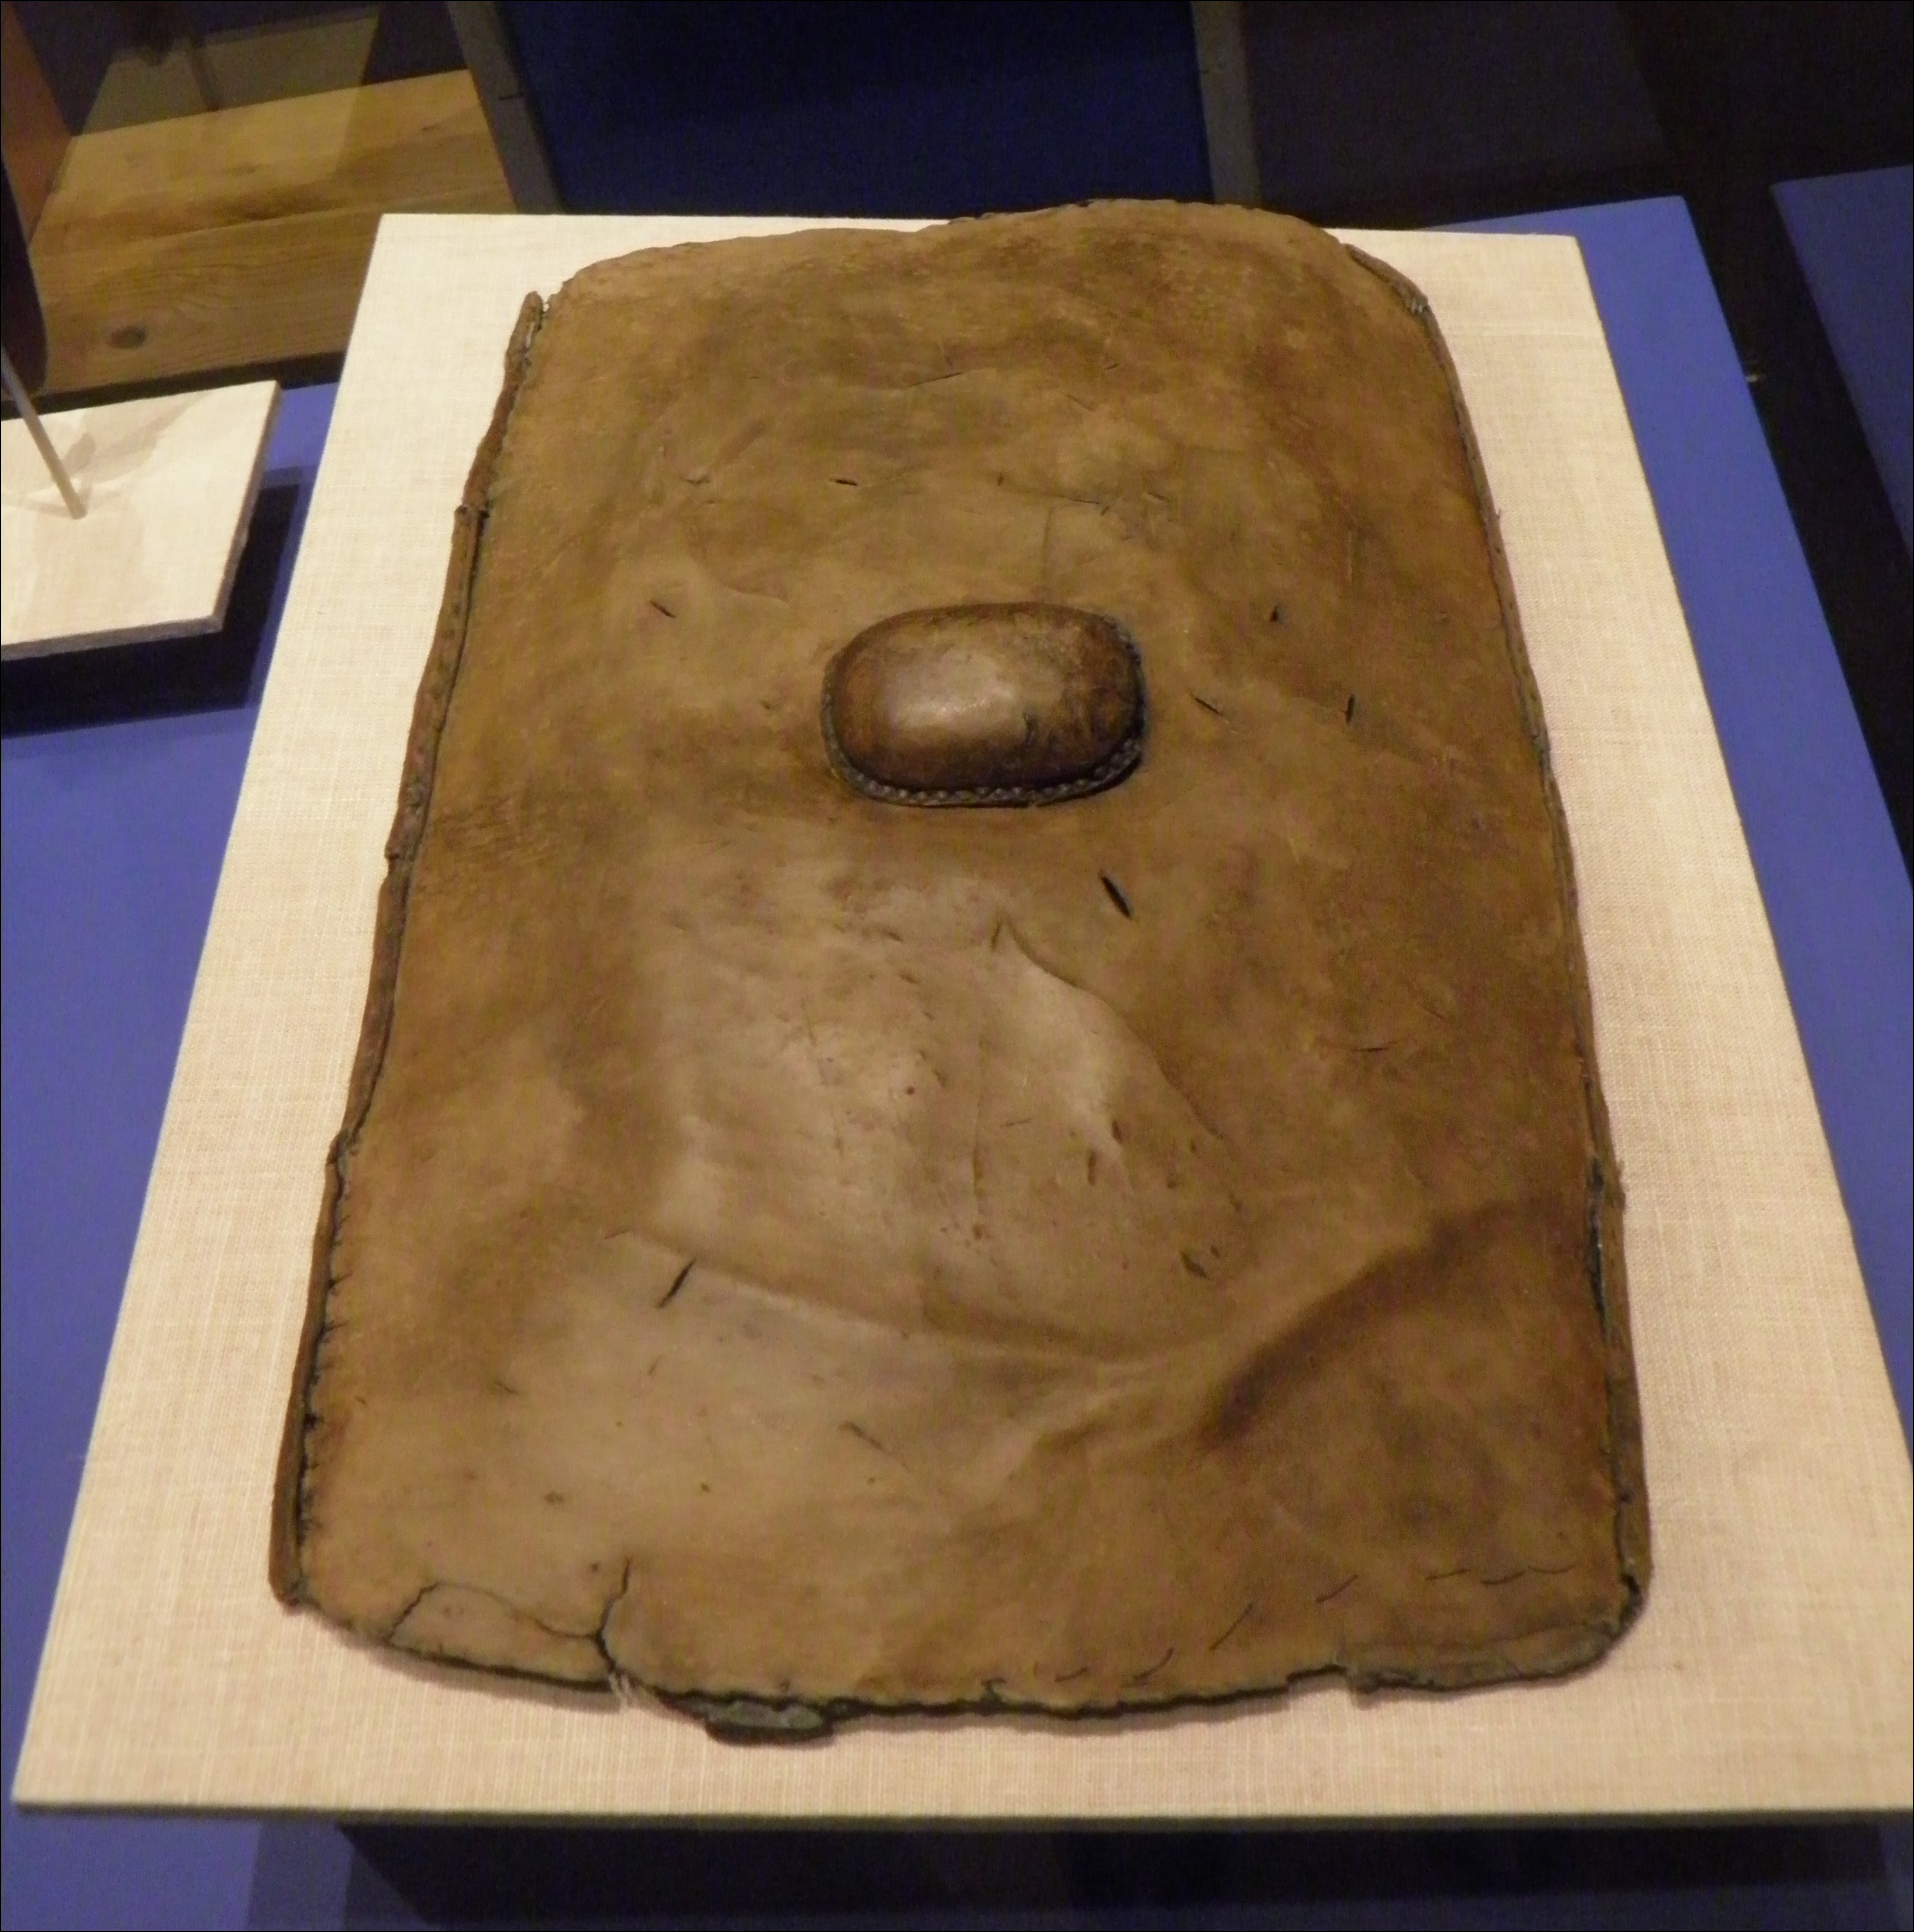
\includegraphics[width=\linewidth]{figures/Hughes_Sword_fig08.jpg} 
\caption{Leather shield from Clonoura bog © Hughes 2015}
\label{hughes_fig8}
\end{wrapfigure}
Like the swords, the Irish shield is smaller than its continental La Tène counterparts, which measured between \SI{110}{\cm} and \SI{120}{\cm} in height \parencite[165]{Lejars2007}. 
Without experimental work we cannot predict its behaviour in use, but one could speculate that it must have been a fairly maneuverable piece of equipment. 
This would indicate that despite the resemblance in size of Irish swords to the Roman \emph{gladius}, the Irish were not engaged in similar heavy infantry tactics requiring a large shield like the Roman scutum. 
Even so, evidence of this shield’s effectiveness in battle is provided by the extensive damage across the front side (fig. \ref{hughes_fig8}).





The overall form of the Irish Iron Age swords informs us that it was probably a close-quarters thrust-and-cut weapon, probably used by infantry, who may also have been armed with a small, manoeuvrable shield and a thrusting spear. This is in comparison to their continental and British contemporaries, the Roman military, while using a short sword, would also have been armed with a much larger shield, and the La Tène Iron Age peoples of the continent would have fought with much bigger shields and longer, slashing swords, albeit with some shorter weapons also in use.

%\subsection{Ireland, the Iron Age and Beyond}
It\marginnote{Ireland, the Iron Age and Beyond} might seem strange that Ireland would have such different weapons and possibly military tactics from Britain and the continent. 
However, there is a period where the fighting style we see in the Irish Iron Age might be paralleled: 
the Irish Bronze Age. The ‘true sword’ as opposed to the so-called rapiers of earlier periods was introduced to Ireland in the earliest part of the Late Bronze Age \parencite[132\psq]{Mallory2013}. These swords vary in length more than those of the Iron Age: they range from \SI{43.5}{\cm} to up to \SI{75.6}{\cm} but many are described as being “...noticeably short” \parencite[52]{Colquhoun2011} and \textcite[105]{Molloy2007} gives \SIrange{400}{600}{\mm} as a range for the early ‘Ballintober’ type, which had a hilt similar to the earlier rapiers but a leaf shaped blade making it more suitable for cutting as well as thrusting.
Irish Iron Age swords would be within the lower end of this range for the most part, but still within it. 
\textcite[105--107]{Molloy2007}  also demonstrates that these weapons would be lethal delivering either cut or thrust. 
Adding to this parallel is the fact that Irish Bronze Age shields,
 though round rather than rectangular are similar in surface area to the Clonoura Iron Age shield (which has a surface area of roughly \SI{1.9}{\meter\squared}). 
An example of a leather Bronze Age shield from Clonfin has a diameter of ca.\,\SI{50}{\cm} \parencite[25]{Osgood2001} giving it a surface area of roughly \SI{1.95}{\meter\squared}.

These similarities could mean that even when a new type of weapon was introduced to Ireland – first the La Tène and later the Roman sword – 
it was adapted to fit the fighting style already in place. 
Horn’s analysis of use-wear on Bronze Age weapons from Nordic countries showed that despite changes in weapon type over time, the type of damage sustained changed very little. 
This indicated that weapons were adapted to suit the type of combat already in place, rather than the other way around \parencite[111\psq]{Horn2013}. 
Perhaps Irish Iron Age combat, instead of moving with the times and evolving toward the long-sword tactics of the continental peoples, retained a more ‘Bronze Age’ fighting style. 
This model of Irish warfare raises questions about other aspects of Irish Iron Age society. 
The most numerous types of La Tène metalwork found in Ireland are objects associated with horse-riding or -driving \parencite[178]{Mallory2013} and \textcite[368]{Dolan2014} highlights the importance the horse must have had to Irish Iron Age society on the basis of this equipment. 
Why then, is there an apparent lack of swords that would be useable from horseback or in a chariot, such as the ones in use on the Continent? 
The lack of differentiated sword types in Ireland might further indicate that we might be seeing a single infantry soldier type in the Irish archaeological record when on the continent, there appears to be a move toward a differentiation between infantry and cavalry \parencite[160]{Lejars2007}, 
something which in turn could be indicative of differing social and economic status.

While the differences between the Irish and British/continental material have been the focus of this study, it also shows us the type of interaction the Irish had with outside areas: 
The Ballyshannon Bay hilt provides evidence for Irish contact with the continent and it should be noted that this is not the only imported material in the area. 
Pottery from the same region of South-west France where the sword hilt probably originated from was dredged up off the Pocupine Bank, off the coast of Co. Sligo, to the south of Ballyshannon bay \parencites[193]{OBrien2009}[25\psq]{CahillWilson2014}. 
This indicates that imported goods could travel to all parts of the country, and were not the preserve of the east coast, where most continental material is found.
As has been outlined above, the anthropoid-hilt sword type is known for its short length compared to other continental La Tène swords, measuring between \SI{29}{\cm} and \SI{55}{\cm} \parencite[69]{Pleiner1993}. 
The fact that this was the type of sword selected for import to Ireland emphasizes the conscious choices of the Irish when it came to the weaponry they used. 
The small number of ‘sub-Roman’ swords in this study also provides evidence for links with the continent, but of a more varied nature. 
The \emph{gladius} type swords found in Ireland are well within their typical range, and may have been imported directly. 
The \emph{spatha} types, on the other hand, have been downsized to “Irish proportions”. That is \SIrange{41}{57}{\cm} in the examples from Lagore compared to \SIrange{65}{90}{\cm} in the Roman world \parencite[48]{Dixon1997}. 
This would seem to indicate that these swords were possibly a local production, inspired by the foreign Roman types but adapted to the conditions of Irish warfare.


%\section{Conclusion}
This\marginnote{Conclusion} project set out to investigate hypothesis that Irish Iron Age swords were suited to a different style of warfare than their continental counterparts, and to challenge the idea that they were ineffective combat tools that would only have been useful in a “...pub brawl” \parencite[65]{Scott1990}. 
This research brought the assemblage of Iron Age swords up to date through survey of the National Museum of Ireland’s single finds and published excavation finds, creating a more representative sample with which to work. 

This allowed the comparison of each sword by dimension, blade shape and blade cross-section. 
It shows that a large proportion of these swords have specific characteristics that allow them to withstand thrusting-type attacks as well as cutting or slashing blows. 
When compared with fighting styles from the continent, such as that of other La Tène Iron Age areas and the Roman military, it would seem that the Irish had a distinct style of warfare.
This ‘Insular fighting style’ may have been based on the type of combat pursued in the Bronze Age: new material imported from the Continent, be it La Tène or Roman in origin, was incorporated into the local fighting style. 

In the case of La Tène weapons and the Roman \emph{spatha}, this was done by making shortened versions of the weapon. There was no need to shorten the anthropoid-hilted sword from Ballyshannon or the Roman \emph{gladius} type swords however, as these weapons were already suited to the type of use the Irish had in mind. 
Together, the short length and blade properties seem to indicate that the Irish Iron Age sword was not designed for use on horseback, but was an effective infantry weapon and not only the preserve of ‘Pub brawls’.
\vspace{2em}
\begin{center}
	* * *
\end{center}
\vspace{2em}
%\section{Acknowledgements}
This\marginnote{Acknowledgements} paper is based on the research undertaken for my undergraduate dissertation as part of my BA in Archaeology in University College Dublin. I would like to thank Dr Alan Peatfield (University College Dublin) for his advice, supervising this research and helping me gain access to the museum collections; Dr Andrew Halpin from the National Museum of Ireland for both his help in accessing the swords and his valuable insights; Dr Greer Ramsey from the Ulster Museum for giving me access to both museum collections and the external storage. Further thanks must go to Dr Barry Molloy and Mr Conor McDermott (University College Dublin), Prof Jim Mallory (Queen’s University Belfast) and Dr Jacqueline Cahill Wilson (University of Bristol) for their valuable advice and support. 
%----------------------------------------------------------------------------------
\clearpage
\begin{myabstract}
\foreignlanguage{french}{%
	Les\marginnote{Abstract (French)}  épées irlandaises de l’âge de fer sont remarquables parce qu’elles sont plus courtes que leurs contemporaines découvertes en Grande Bretagne et en Europe continentale à l’époque de La Tène. C’est à cause de cette caractéristique que l’on a émis l’hypothèse qu’elles étaient essentiellement des sortes de poignards ou des objets de cérémonie qui n’étaient pas destinés au combat. La présente recherche intègre des études d’épées précédemment publiées à du nouveau matériel provenant de l’étude de bases de données de musées irlandais, et a pour but d’examiner les épées en termes de morphologie et de dimension de lame, et d’en déduire leur utilisation possible dans les batailles. L’étude montre que la majorité des épées de la période 700 avant J.C.- 400 apr. J.C., qu’elles soient de type La Tène ou sub-romain, ont des caractéristiques d’armes utilisées pour se battre à pied.  Ceci est en désaccord avec la nature des armes découvertes ailleurs à la même époque en Grande Bretagne et en Europe continentale, et souligne le développement insulaire de l’Irlande durant cette période. À travers deux études de cas, la présente analyse montre également qu’interagir avec le monde extérieur a pu signifier choisir d’importer des armes et des idées. Le présent article clarifie les suggestions indiquées dans d’autres travaux relatifs aux utilisations de ces épées et examine les épées sous un autre angle, l’angle sous lequel ces armes se rattachent à la nature même de la guerre et de la société dans l’Irlande de l’âge de fer.}
\end{myabstract}

\begin{center}
	* * *
\end{center}%
%\subsection*{Abbreviations used in Appendix 1}
%\begin{description}
%	\setlength{\itemsep}{0pt}%
%	\setlength{\parskip}{0pt}%
%	\setlength{\parsep}{0pt}%
%\item[BM]British Museum
%\item[NMI]		National Museum of Ireland
%\item[UCMAE]	University of Cambridge Museum of Archaeology and Ethnography
%\item[UM]		Ulster Museum
%\end{description}

%\protect\alertinfo{
\textbf{\sffamily Abbreviations used in Appendix 1:} 
	\begin{labeling}{UCMAE}\setlength{\itemsep}{0pt}\setlength{\parskip}{0pt}\setlength{\parsep}{0pt}%
		\item[BM] British Museum
		\item[NMI]		National Museum of Ireland
		\item[UCMAE]	University of Cambridge Museum of Archaeology and Ethnography
		\item[UM]		Ulster Museum
	\end{labeling}
%}
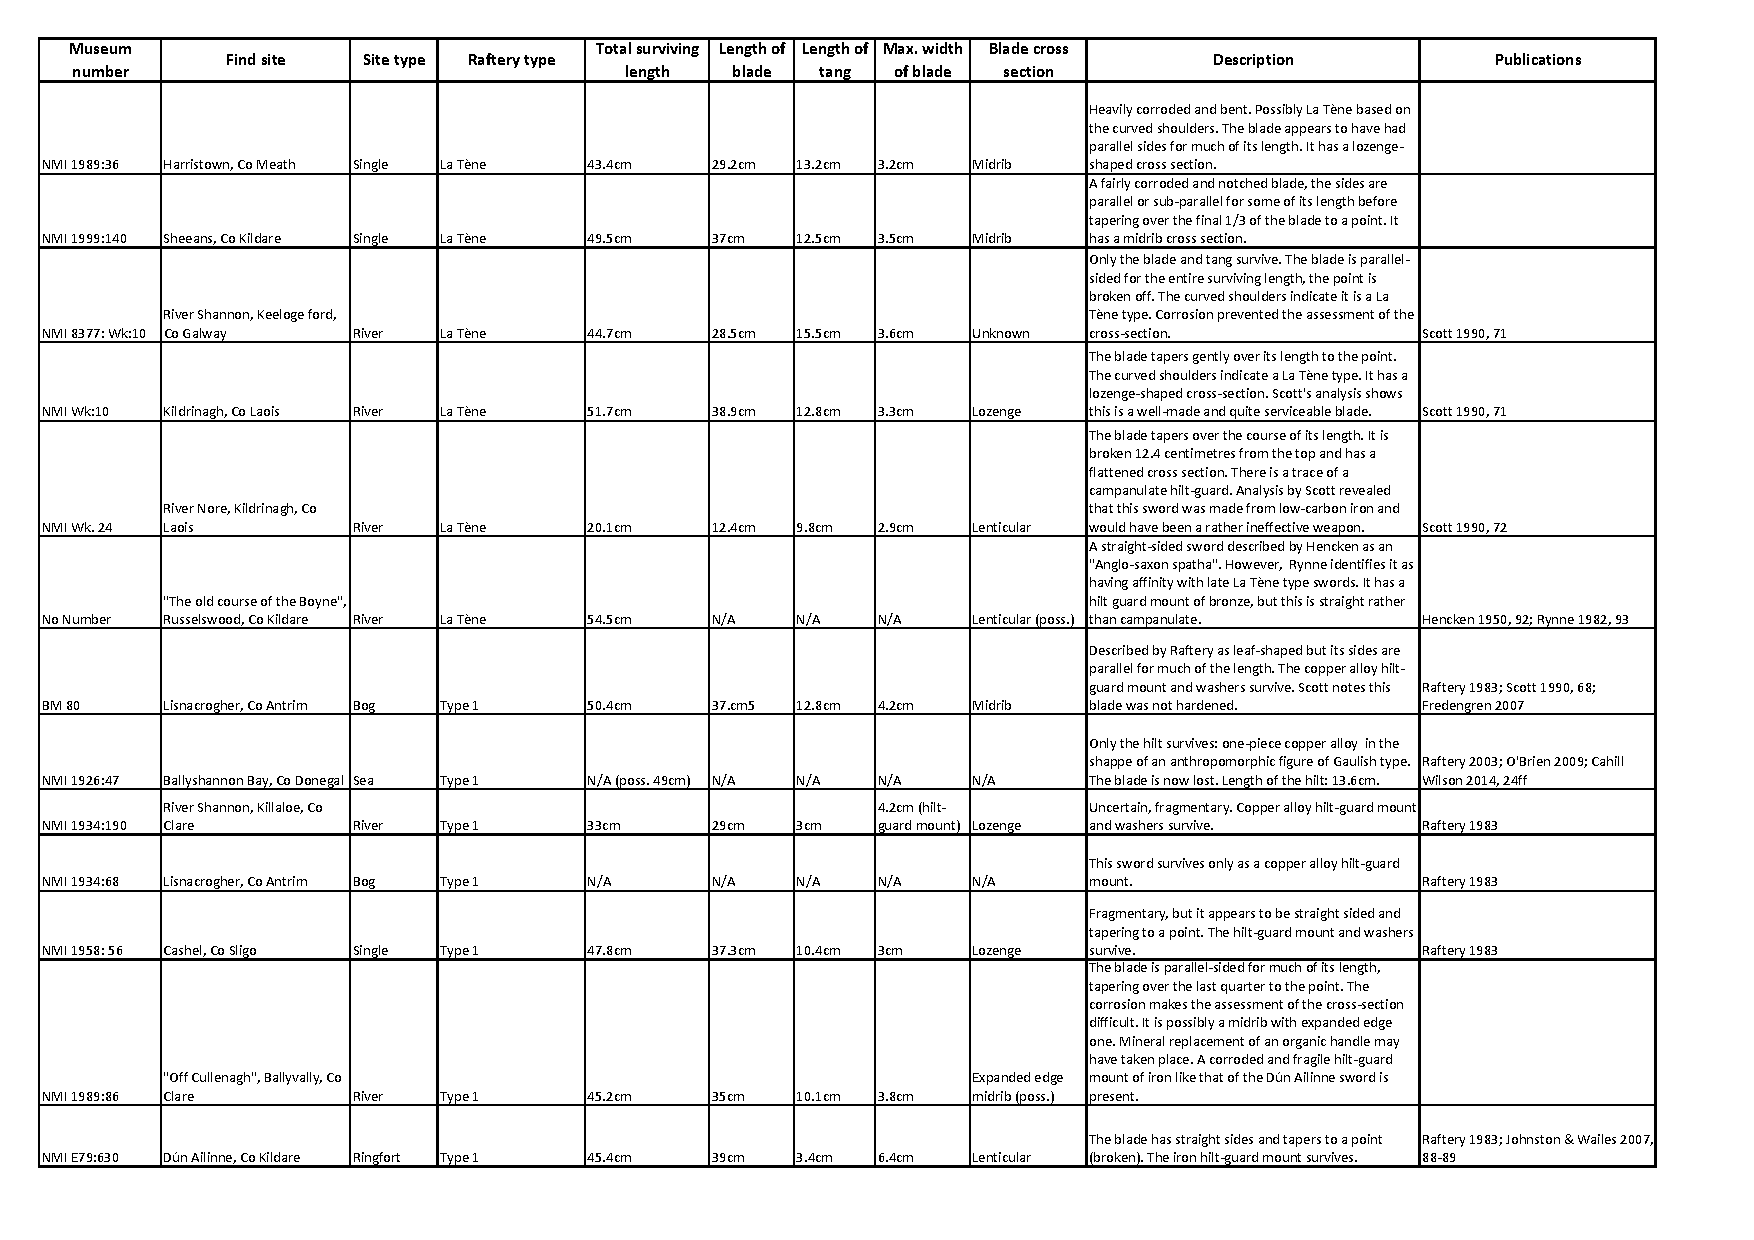
\includepdf[landscape=true,pages=-]{figures/Hughes_Sword_appendix} 


\printbibliography[heading=subbibnumbered] 

\label{hughes:lastpage}
\sisetup{%
	range-phrase ={$\times$},%
}
%----------------------------------------------------------------------------------
\closingarticle